\chapter{The Translating Coil Fluxmeter}
The magnetometer consists of several components. A PCB with 
printed flux pickup coils, fast digital integrators, a rotary
encoder and a laser tracker system for geometric positioning measurements.
Strictly, the laser tracker is not required, as the encoder can be used
for positioning. Still, it was used to increase
the geometrical accuracy.

\begin{figure}[!h]
    \centering
    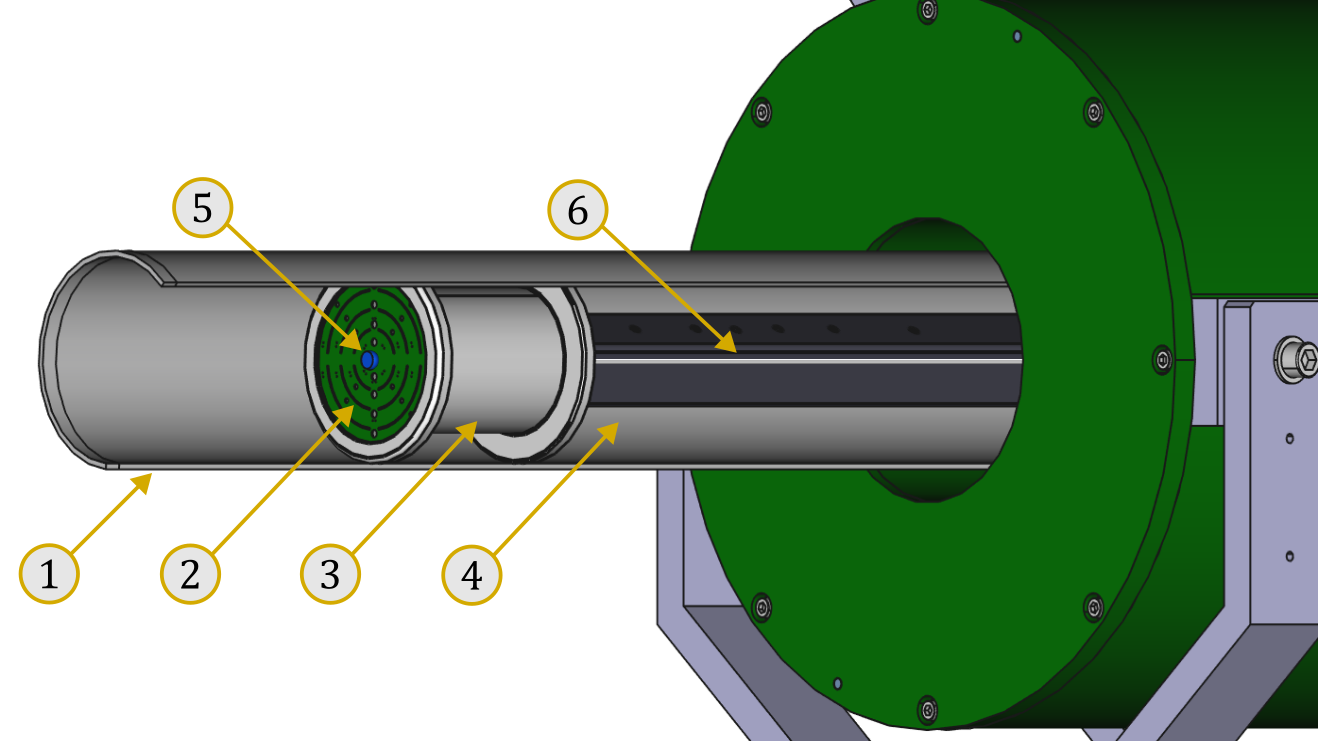
\includegraphics[width=0.7\textwidth]{figs/elena}
    \caption{The fluxmeter assembly going through a solenoid magnet. \\
    1. Guiding Tube, 2. Fluxmeter PCB, 3. PCB Sledge, 4. Supporting arm, 
    5. Laser Reflector, 6. Encoder Wire}
    \label{fig:elena}
\end{figure}

To move the PCB through the magnet aperture, a support assembly was made as
seen in figure \ref{fig:elena}. The coil cables are run through the supporting
arm, which is also used to push and pull the fluxmeter through the tube. A 
wire is connected to the PCB sledge on one end, and spooled up around
a rotating encoder on the other end. In the middle of the PCB, a 
reflector was mounted for the laser tracker.

\section{PCB printed coils}
The coil PCB has 21 different coils.
These coils are in the shapes of disks or annulus segments.
A render of the pcb can be seen in figure
\ref{fig:pcb}. The disks are denoted $D_l$ and the 
annulus segments by $Q_{q, l}$ where $l$ is the radial layer and 
$q$ is the quadrant, as seen in figure \ref{fig:nomenclature}.

\begin{figure}[!h]
    \centering
    \begin{subfigure}[b]{0.5\linewidth}
        \centering
        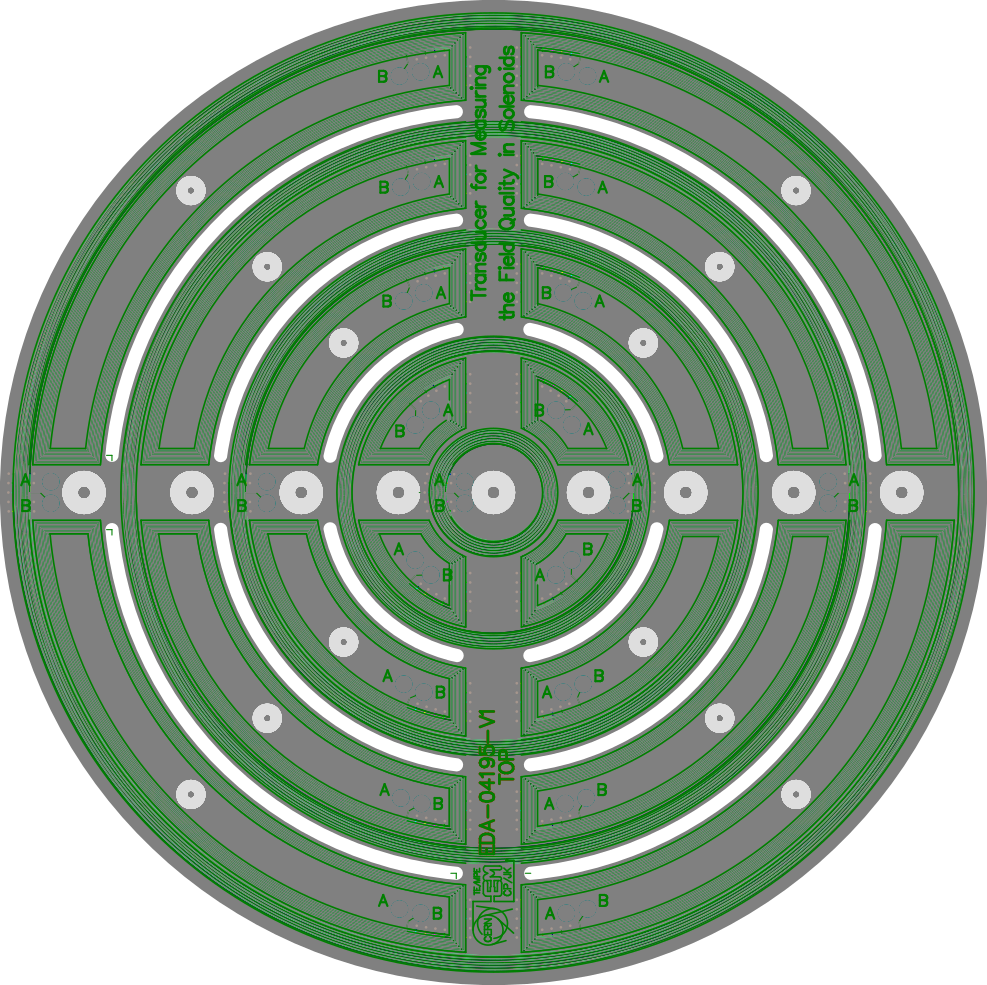
\includegraphics[width=0.8\linewidth]{figs/pcb}
        \caption{The fluxmeter PCB.}
        \label{fig:pcb}
    \end{subfigure}
    \hfill
    \begin{subfigure}[b]{0.4\linewidth}
        \centering
        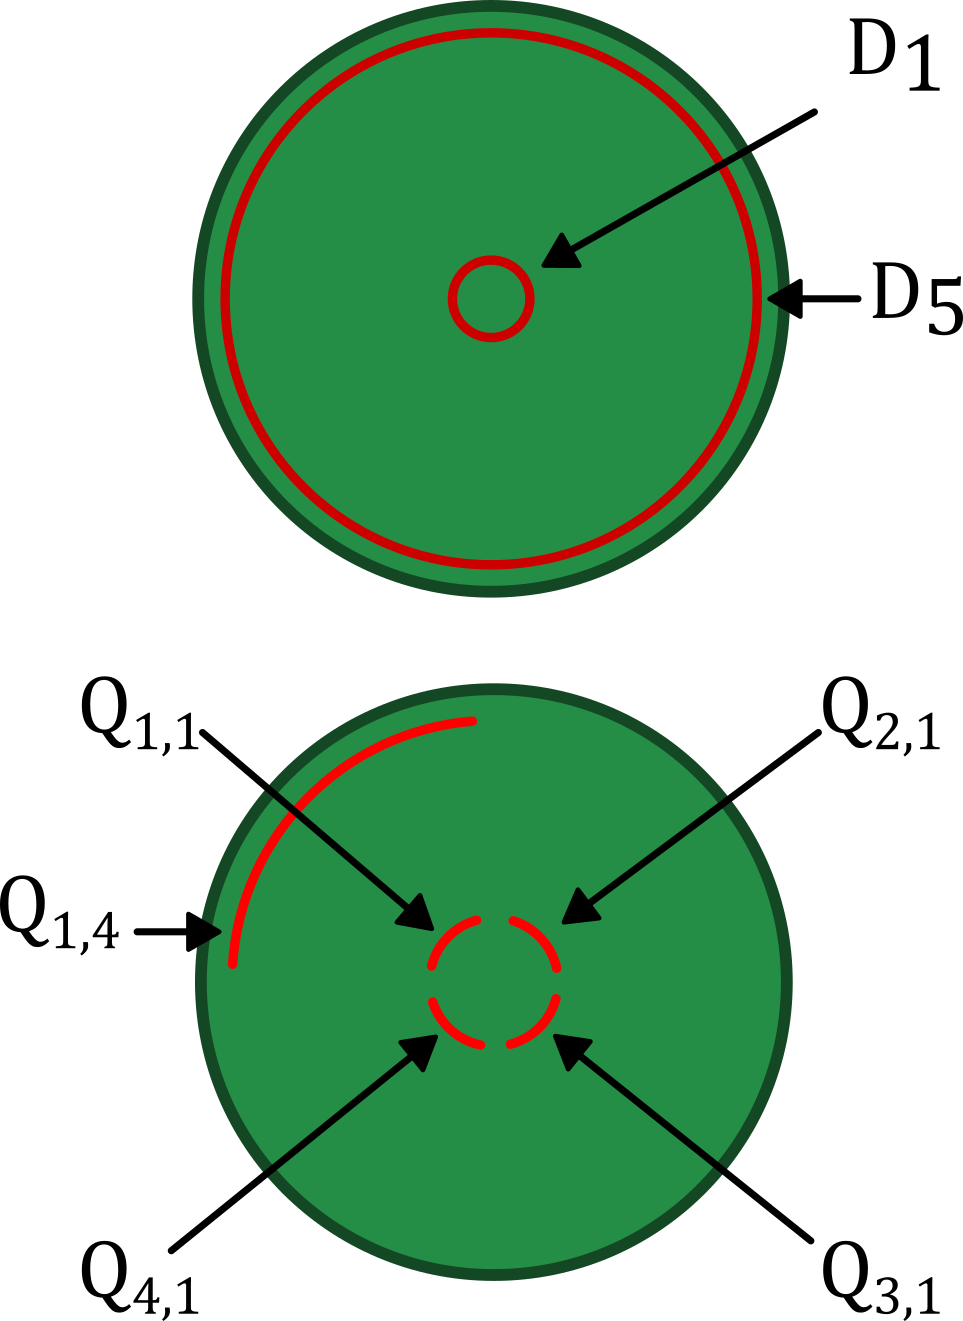
\includegraphics[width=0.8\linewidth]{figs/nomenclature.png}
        \caption{Nomenclature of the PCB coils.}
        \label{fig:nomenclature}
    \end{subfigure}
    \caption{}
\end{figure}

\section{Positional Encoder}
\section{Fast Digital Integrators}
\section{Geometric Lidar Measurements}
\section{The Measurement Assembly}